\section{Chapitre 0 - Calculer avec une machine}
\setcounter{cor}{2}
\begin{cor}[Un premier programme]
\begin{enumerate}
	\item \lstinputlisting[language=Scilab]{00-Calculer-avec-une-machine/Scripts-Scilab/ex3-Heron1.sci}
			Pour obtenir une plus grande pr�cision, on demandera plus de d�cimal avec la fonction \textbf{format}. Par d�faut elle est de 10 d�cimales affich�es. La pr�cision maximale est de l'ordre de 16 d�cimales. On constate que la convergence de la m�thode est tr�s rapide.\\
\begin{lstlisting}
-->format(20)
-->Heron1(2,10)
 ans  =
    1.41421356237309492  
-->Heron1(16,6)
 ans  =
    4.00000000000005063  
-->Heron1(16,7)
 ans  =
    4.  
 \end{lstlisting}
\item Pour garder en m�moire les r�sultats il vaut mieux travailler avec une matrice.\\
			\lstinputlisting[language=Scilab]{00-Calculer-avec-une-machine/Scripts-Scilab/ex3-Heron2.sci}
			
			\newpage
			En testant \textbf{Heron2(16,10)} on obtient :
			\begin{center}
				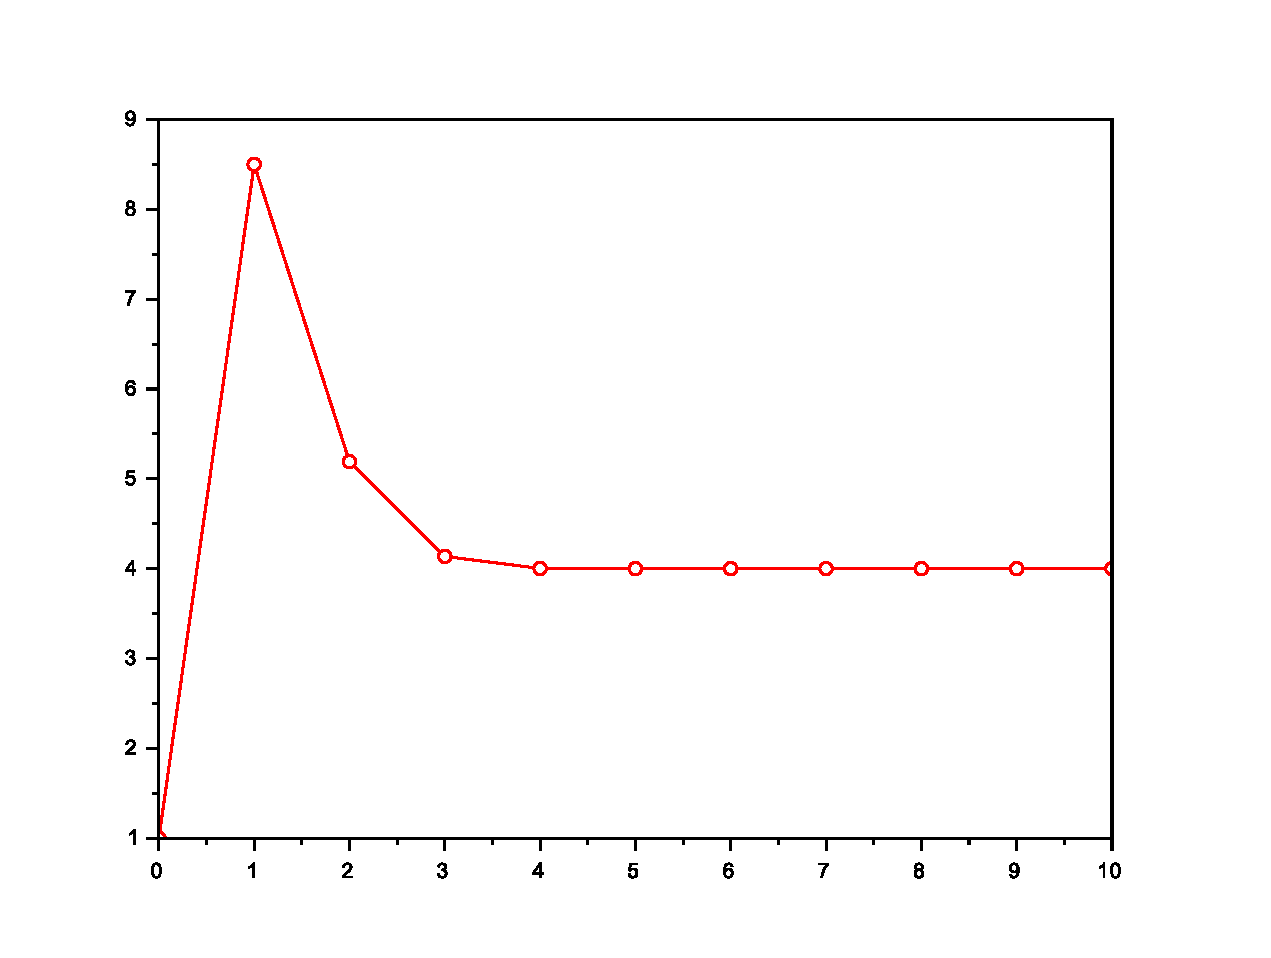
\includegraphics[scale=0.5]{00-Calculer-avec-une-machine/Scripts-Scilab/ex3-heron2-racine4.pdf}
			\end{center}

\item \lstinputlisting[language=Scilab]{00-Calculer-avec-une-machine/Scripts-Scilab/ex3-Heron3.sci}
			En testant \textbf{Heron3(2,\%eps)} on obtient le r�sultat 1.41421356237309492 pour $n=5$ et le graphe suivant :
			\begin{center}
				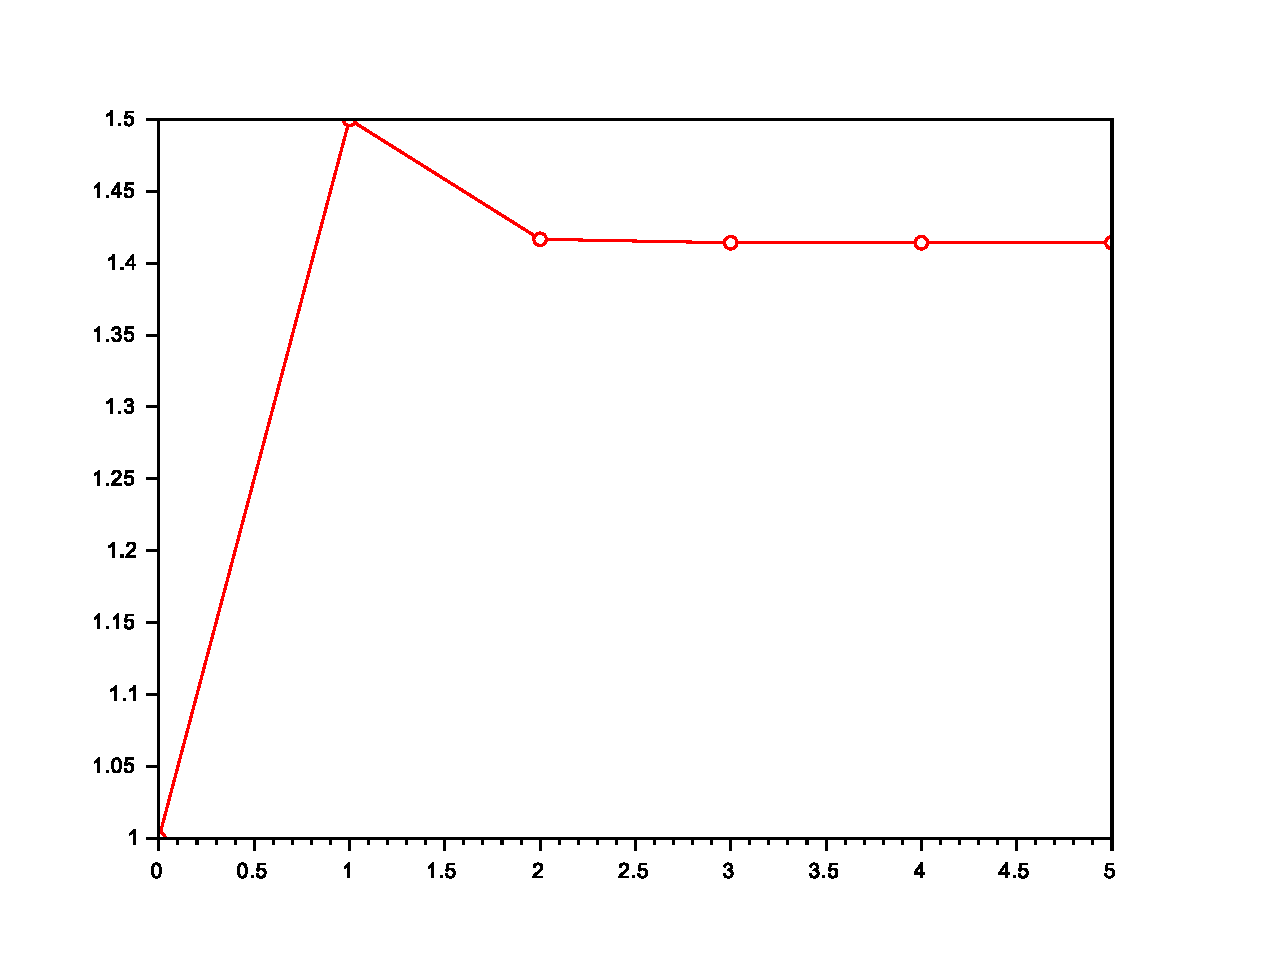
\includegraphics[scale=0.5]{00-Calculer-avec-une-machine/Scripts-Scilab/ex3-heron3-racine2.pdf}
			\end{center}

\end{enumerate}
\end{cor}